\documentclass[conference]{IEEEtran}
\IEEEoverridecommandlockouts

\usepackage[utf8]{inputenc}
\usepackage[T1]{fontenc}
\usepackage[portuguese]{babel}
\usepackage{cite}
\usepackage{amsmath,amssymb,amsfonts}
\usepackage{graphicx}
\usepackage{booktabs}
\usepackage{textcomp}
\usepackage{xcolor}
\usepackage{url}

\def\BibTeX{{\rm B\kern-.05em{\sc i\kern-.025em b}\kern-.08em
    T\kern-.1667em\lower.7ex\hbox{E}\kern-.125emX}}

\begin{document}

\title{StratGraph: Otimiza\c{c}\~ao de Rotas Estrat\'egicas via Grafo Ponderado Expandido em Camadas e Contra\c{c}\~ao Topol\'ogica}

\author{
\IEEEauthorblockN{Heitor Henrique Zonho\IEEEauthorrefmark{1},
Kairo Henrique Ferreira Martins\IEEEauthorrefmark{1},
Michel Pires da Silva\IEEEauthorrefmark{1}}
\IEEEauthorblockA{\IEEEauthorrefmark{1}Engenharia de Computa\c{c}\~ao --- Universidade Federal de Ci\^encia e Inova\c{c}\~ao de Minas Gerais (UFCI-MG)\\
Divin\'opolis, Brasil}
}

\maketitle

\begin{abstract}
O planejamento de trajet\'orias em ambientes com desvios estrat\'egicos exige equilibrar o custo real de deslocamento, a aquisi\c{c}\~ao de equipamentos que reduzem riscos futuros e a coleta de recompensas opcionais. Algoritmos cl\'assicos sobre grafos est\'aticos ignoram redu\c{c}\~oes din\^amicas de dificuldade ap\'os a coleta de recursos ou geram ciclos negativos ao subtrair b\^onus das arestas. Este trabalho apresenta o \textit{StratGraph}, um motor gen\'erico em Python~3.12 para grafos dirigidos com expans\~ao em duas camadas de estado ($L_0$ sem recurso e $L_1$ com recurso), contra\c{c}\~ao iterativa de becos sem sa\'ida e fun\c{c}\~ao substituta heur\'istica estritamente positiva. A abordagem \'e validada em 14 mapas extra\'idos de \textit{Celeste} (8 cap\'itulos) e \textit{Cuphead} (6 fases), al\'em de 7 benchmarks sint\'eticos e an\'alise estrutural no Gephi. O algoritmo de Dijkstra em camadas otimiza exatamente o objetivo substitutivo est\'atico sobre $G_L$ em tempo polinomial $O((V+E)\log V)$, sendo comparado \`a Busca em Largura (BFS) e ao \textit{Branch-and-Bound} em profundidade (DFS). Nos experimentos, a contra\c{c}\~ao absorve at\'e 72,7\% dos v\'ertices e garante 100\% dos colet\'aveis situados em alcovas terminais (100\% do mapa nas 14 fases reais), enquanto o Dijkstra em camadas reduz o custo real de travessia em at\'e 50,9\% em \textit{Celeste} e 68,3\% em \textit{Cuphead} frente ao BFS, resolvendo 5.000 salas em 14,49~ms.
\end{abstract}

\begin{IEEEkeywords}
Teoria dos grafos, grafo em camadas, caminho m\'inimo, algoritmo de Dijkstra, an\'alise topol\'ogica, Gephi.
\end{IEEEkeywords}

% ============================================================================
\section{Introdu\c{c}\~ao}
% ============================================================================

O planejamento automatizado de rotas em grafos ponderados constitui um problema fundamental na ci\^encia da computa\c{c}\~ao, abrangendo desde roteamento log\'istico e rob\'otica m\'ovel at\'e a intelig\^encia artificial aplicada a jogos digitais. Nesses dom\'inios, entretanto, o custo de transpor uma conex\~ao frequentemente n\~ao \'e fixo: a obten\c{c}\~ao pr\'evia de uma ferramenta, habilidade ou \textit{power-up} em um setor secund\'ario reduz substancialmente a dificuldade de todo o percurso restante, ao mesmo tempo em que alcovas opcionais concentram itens colet\'aveis desej\'aveis para metas de pontua\c{c}\~ao integral (\textit{All Collectibles}).

Quando modelado diretamente sobre um d\'igrafo est\'atico convencional, o problema sofre de duas limita\c{c}\~oes cl\'assicas. Abordagens baseadas em saltos m\'inimos, como a Busca em Largura (BFS), ignoram tanto pesos heterog\^eneos quanto a mudan\c{c}a de estado ap\'os a aquisi\c{c}\~ao de equipamentos. Por outro lado, tentar embutir b\^onus de colet\'aveis subtraindo-os aditivamente dos pesos das arestas produz custos negativos ou ciclos atrativos que violam a pr\'e-condi\c{c}\~ao de n\~ao negatividade do algoritmo de Dijkstra~\cite{dijkstra1959,cormen2022}. Al\'em disso, modelar integralmente o hist\'orico de todos os $k$ itens coletados no espa\c{c}o de estados conduz \`a explos\~ao combinat\'oria $O(2^k|V|)$, aproximando-se de variantes NP-dif\'iceis como o \textit{Prize-Collecting Traveling Salesman Problem} (PCTSP) e o \textit{Orienteering Problem}~\cite{balas1989,vansteenwegen2011}.

Diante desse cen\'ario, a motiva\c{c}\~ao deste trabalho \'e construir um n\'ucleo algor\'itmico inteiramente agn\'ostico a dom\'inio --- execut\'avel via terminal Linux apenas com a biblioteca padr\~ao do Python~3.12 --- capaz de conciliar o desvio estrat\'egico por recursos, a captura sistem\'atica de alcovas colet\'aveis e a efici\^encia polinomial, utilizando datasets extra\'idos de n\'iveis comerciais e grafos sint\'eticos como benchmarks emp\'iricos reprodut\'iveis. Os objetivos espec\'ificos s\~ao: (i) formalizar e implementar o pr\'e-processamento por contra\c{c}\~ao de becos sem sa\'ida e a expans\~ao em duas camadas ($L_0 \to L_1$) sob uma fun\c{c}\~ao substituta heur\'istica estritamente positiva; (ii) analisar visual e metricamente as redes geradas no Gephi~\cite{bastian2009} por modularidade e grau; e (iii) comparar experimentalmente BFS, DFS \textit{Branch-and-Bound} e Dijkstra em camadas quanto ao custo real de travessia, peso efetivo, coleta de itens e escalabilidade at\'e $|V|=5.000$.

O restante deste artigo est\'a organizado da seguinte forma. A Se\c{c}\~ao~\ref{sec:referencial} revisa o referencial te\'orico sobre caminhos m\'inimos e roteamento sens\'ivel a estado. A Se\c{c}\~ao~\ref{sec:metodologia} descreve a metodologia modular do \textit{StratGraph}, as decis\~oes de projeto e o fluxo no Gephi. A Se\c{c}\~ao~\ref{sec:resultados} apresenta e discute os resultados quantitativos e topol\'ogicos, os gargalos observados e a an\'alise de sensibilidade. A Se\c{c}\~ao~\ref{sec:conclusao} sintetiza conclus\~oes, limita\c{c}\~oes e trabalhos futuros, e a Se\c{c}\~ao~\ref{sec:disponibilidade} detalha os reposit\'orios do algoritmo e da base de dados.

% ============================================================================
\section{Referencial Te\'orico}
\label{sec:referencial}
% ============================================================================

O problema de caminho m\'inimo de fonte \'unica em d\'igrafos com pesos n\~ao negativos possui solu\c{c}\~ao cl\'assica pelo algoritmo guloso de Dijkstra~\cite{dijkstra1959}. Empregando fila de prioridade bin\'aria (\textit{min-heap}), sua complexidade de tempo \'e limitada por $O((V + E)\log V)$, enquanto a Busca em Largura (BFS) executa em $O(V + E)$, por\'em minimiza apenas a cardinalidade de arestas em grafos n\~ao ponderados~\cite{cormen2022}.

Em planejamentos nos quais o custo ou a viabilidade de transi\c{c}\~oes depende do estado de invent\'ario do agente, configura-se o problema de \textit{Inventory-Aware Pathfinding}. Aversa et al.~\cite{aversa2016} demonstram que incorporar vari\'aveis de invent\'ario ao v\'ertice preserva a propriedade de Markov sobre um grafo de estados expandido, evitando rec\'alculos din\^amicos por aresta, mas destacam que t\'ecnicas pr\'evias de poda e redu\c{c}\~ao topol\'ogica s\~ao essenciais para conter o crescimento do grafo expandido.

De modo complementar, a inclus\~ao seletiva de v\'ertices opcionais portadores de recompensa relaciona-se diretamente ao \textit{Prize-Collecting Traveling Salesman Problem} (PCTSP) formulado por Balas~\cite{balas1989} e ao \textit{Orienteering Problem} revisado por Vansteenwegen et al.~\cite{vansteenwegen2011}, ambos NP-dif\'iceis em grafos gerais. No \textit{StratGraph}, adota-se uma relaxa\c{c}\~ao markoviana polinomial de estado \'unico bin\'ario ($k \in \{0,1\}$) combinada \`a contra\c{c}\~ao pr\'evia de alcovas sem sa\'ida e \`a explora\c{c}\~ao visual de comunidades e graus ponderados via Gephi~\cite{bastian2009}.

% ============================================================================
\section{Metodologia}
\label{sec:metodologia}
% ============================================================================

A Figura~\ref{fig:fluxograma} sintetiza as cinco etapas do pipeline modular implementado em Python~3.12 (biblioteca padr\~ao em \texttt{src/}), projetado de forma gen\'erica para aceitar qualquer grafo dirigido no formato padronizado (\texttt{vertices.csv} e \texttt{arestas.csv}).

\begin{figure}[htbp]
\centering
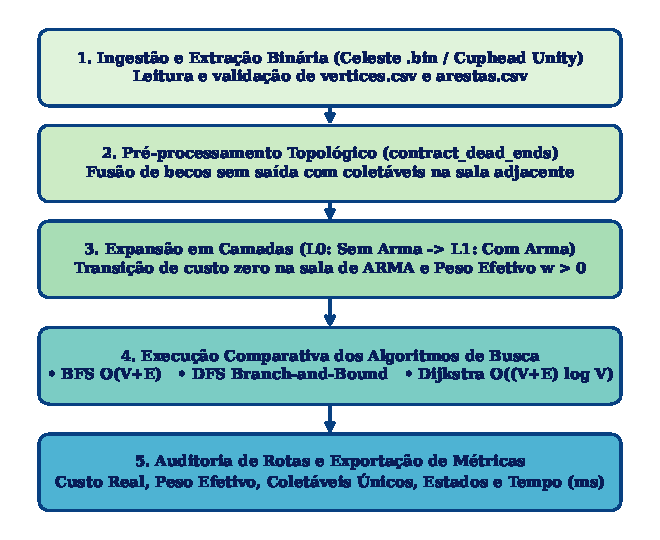
\includegraphics[width=\columnwidth]{figures/fluxograma_proposta.pdf}
\caption{Fluxograma completo da metodologia do \textit{StratGraph}, da ingest\~ao gen\'erica em CSV \`a auditoria comparativa e exporta\c{c}\~ao topol\'ogica.}
\label{fig:fluxograma}
\end{figure}

\subsection{Arquitetura Modular e Ingest\~ao dos Benchmarks}
O n\'ucleo em \texttt{src/} \'e totalmente desacoplado de motores espec\'ificos e organiza-se em cinco m\'odulos principais: \texttt{src/models.py} (estruturas de dados \texttt{Vertex}, \texttt{Edge}, \texttt{GameGraph}, \texttt{LayeredNode} e \texttt{RouteResult}), \texttt{src/loader.py} (valida\c{c}\~ao e leitura dos arquivos CSV), \texttt{src/preprocessing.py} (contra\c{c}\~ao topol\'ogica iterativa), \texttt{src/layered\_graph.py} (expans\~ao em camadas e pondera\c{c}\~ao heur\'istica) e \texttt{src/algorithms.py}/\texttt{src/metrics.py} (executores de busca e c\'alculo de m\'etricas). Como benchmarks emp\'iricos externos ao n\'ucleo, utilizaram-se tr\^es fam\'ilias de grafos documentadas em~\cite{dataset_zenodo}:
\begin{itemize}
    \item \textbf{\textit{Celeste} (8 cap\'itulos oficiais):} Extrator dedicado decodifica o formato bin\'ario \texttt{BinaryPacker} (\texttt{.bin}) da \textit{engine} Monocle dos cap\'itulos 1 (\textit{Forsaken City}) a 9 (\textit{Core}), utilizando busca $A^*$ no grid de colis\~ao $8\times 8$ (\texttt{solids}) para estimar custos intra-sala entre portas e colet\'aveis (\texttt{strawberry}, \texttt{cassette}, \texttt{blackGem}). Os experimentos consomem exclusivamente os CSVs pr\'e-processados.
    \item \textbf{\textit{Cuphead} (6 fases \textit{Run-and-Gun}):} Extrator sobre os bin\'arios \texttt{SerializedFile} v17 (\texttt{level41} a \texttt{level46}) da Unity obt\'em coordenadas de plataformas, as 5 moedas douradas (\texttt{Level\_Coin}) e exposi\c{c}\~ao a \textit{spawners} de inimigos com e sem melhoria de ataque (\textit{parry/arma}).
    \item \textbf{Benchmarks Sint\'eticos:} Gerador determin\'istico para $|V| \in \{15, 30, 60, 150, 500, 1500, 5000\}$, contendo 20\% de alcovas colet\'aveis em beco sem sa\'ida e atalhos com ciclos paralelos para avalia\c{c}\~ao de escalabilidade.
\end{itemize}

\subsection{Contra\c{c}\~ao de Becos e Expans\~ao Markoviana em Camadas}
Seja $G = (V, E)$ o d\'igrafo de entrada. No m\'odulo \texttt{src/preprocessing.py} (\texttt{contract\_dead\_ends}), uma sala $c \in V \setminus \{v_{\text{ini}}, v_{\text{fim}}\}$ sem arma e conectada bidirecionalmente a um \'unico vizinho $b$ (desde que $b$ n\~ao seja sala de arma, podendo inclusive ser $v_{\text{ini}}$ ou $v_{\text{fim}}$) \'e contra\'ida iterativamente em $b$: folhas vazias s\~ao podadas e alcovas com $\text{ValorColetavel}(c) > 0$ transferem seu valor para $b$, somando o menor custo de ida e volta $(b \to c \to b)$ de forma independente para as camadas sem arma e com arma nas arestas incidentes em $b$, registrando a auditoria em \texttt{contracted\_into[$b$]}. Assumiu-se explicitamente esta contra\c{c}\~ao como decis\~ao de projeto alinhada \`a meta \textit{All Collectibles} nas ramifica\c{c}\~oes terminais, obrigando qualquer rota que atravesse o n\'o pai $b$ a capturar suas folhas associadas.

Sobre o grafo reduzido $G' = (V', E')$, o m\'odulo \texttt{src/layered\_graph.py} (\texttt{build\_layered\_graph}) constr\'oi o d\'igrafo expandido $G_L = (V_L, E_L)$ com $V_L = V' \times \{0, 1\}$: $k=0$ representa o estado inicial sem equipamento ($\text{DificuldadeSemArma}$) e $k=1$ o estado com equipamento ($\text{DificuldadeComArma}$). Para cada v\'ertice $u_{\text{arma}}$, adiciona-se a transi\c{c}\~ao $(u_{\text{arma}}, 0) \to (u_{\text{arma}}, 1)$ de custo real zero e peso zero.

Como segunda decis\~ao expl\'icita de projeto, o estado $(v, k)$ n\~ao armazena uma m\'ascara bin\'aria dos colet\'aveis j\'a visitados. Em grafos gerais, rastrear $r$ salas colet\'aveis explodiria o espa\c{c}o de estados para $O(2^r|V|)$; ao manter apenas $k \in \{0,1\}$, preserva-se o porte polinomial $|V_L| = 2|V'|$ como relaxa\c{c}\~ao markoviana trat\'avel. Como terceira decis\~ao de projeto, o atrativo pelos colet\'aveis \'e modelado pela fun\c{c}\~ao substituta heur\'istica estritamente positiva:
\begin{equation}
w(u, v, k) = \frac{\text{TempoBase}(u, v) + \text{Dificuldade}(u, v, k)}{1 + \alpha \cdot \text{ValorColetavel}(v)}, \quad \alpha \ge 0
\label{eq:peso_efetivo}
\end{equation}
na qual o par\^ametro $\alpha$ regula o compromissso entre custo f\'isico e coleta, assegurando $w > 0$ para validade do algoritmo de Dijkstra.

\subsection{Algoritmos Comparados e Auditoria de Rotas}
No m\'odulo \texttt{src/algorithms.py}, tr\^es algoritmos operam sobre $G_L$ a partir de $(v_{\text{ini}}, 0)$:
\begin{enumerate}
    \item \textbf{BFS ($O(V+E)$):} \textit{Baseline} em largura que minimiza apenas o n\'umero de arestas at\'e $v_{\text{fim}}$, ignorando pesos e desvios por arma.
    \item \textbf{DFS \textit{Branch-and-Bound}:} Busca em profundidade exata sobre caminhos simples em camadas (com limite de tempo de 150~ms nos experimentos) e controle de \texttt{seen\_rooms}, evitando reaplicar o desconto de $\text{ValorColetavel}(v)$ caso uma mesma sala seja atravessada em $L_0$ e $L_1$.
    \item \textbf{Dijkstra em Camadas ($O((V+E)\log V)$):} Resolve exatamente a soma aditiva est\'atica dos pesos substitutivos (\ref{eq:peso_efetivo}) sobre $G_L$ com fila de prioridade \texttt{heapq}. Ao final, a fun\c{c}\~ao \texttt{evaluate\_path} calcula tanto o \textbf{custo real} bruto ($\sum (\text{TempoBase}+\text{Dificuldade})$) quanto o \textbf{peso efetivo sem dupla contagem}, distinguindo a relaxa\c{c}\~ao otimizada na busca da avalia\c{c}\~ao consolidada do percurso.
\end{enumerate}

Ainda em \texttt{src/metrics.py}, o c\'alculo de \textit{gap} percentual frente ao \textit{DFS Branch-and-Bound} \'e restringido estritamente aos casos em que o DFS concluiu sem exceder o tempo limite (\texttt{timed\_out = False}), evitando compara\c{c}\~oes esp\'urias ou negativas contra limites parciais interrompidos.

\subsection{Constru\c{c}\~ao e An\'alise Estrutural no Gephi}
Para inspecionar visual e metricamente a topologia antes e depois das transforma\c{c}\~oes, o script \texttt{scripts/export\_gephi.py} exporta cada inst\^ancia e os grafos unificados para o formato GEXF~1.2, compat\'ivel com o software Gephi~\cite{bastian2009}. O fluxo de an\'alise estrutural segue quatro passos: (i) espacializa\c{c}\~ao por for\c{c}as dirigidas (\textit{Force Atlas 2}) para separar o eixo principal das ramifica\c{c}\~oes secund\'arias; (ii) c\'alculo de comunidades via \textit{Modularity Class} (algoritmo de Louvain), grau m\'edio ($k_{\text{m\'ed}}$) e densidade; (iii) escalonamento visual dos n\'os pelo grau e codifica\c{c}\~ao crom\'atica de comunidades, alcovas contra\'iveis e camadas ($L_0$ vs. $L_1$); e (iv) filtragem booleana pelo atributo \texttt{na\_rota\_otima} para isolar visualmente o desvio pela sala de arma frente \`a trajet\'oria direta do BFS.

% ============================================================================
\section{Resultados e Discuss\~ao}
\label{sec:resultados}
% ============================================================================

Os experimentos foram executados integralmente em terminal sem depend\^encia de motores comerciais de jogo, adotando $\alpha = 0{,}05$ e mediana de 5 repeti\c{c}\~oes por inst\^ancia, com \textit{timeout} de 150~ms para o DFS \textit{Branch-and-Bound}.

\subsection{An\'alise Topol\'ogica no Gephi e Contra\c{c}\~ao de Becos}
A Figura~\ref{fig:gephi_macro} ilustra a an\'alise visual e estrutural do cap\'itulo \textit{1-Forsaken City}. No grafo base (Fig.~\ref{fig:gephi_macro}a), a detec\c{c}\~ao de comunidades revela seis blocos modulares ($Q = 0{,}70$), onde os losangos vermelhos evidenciam becos sem sa\'ida perif\'ericos portadores de morangos. Ap\'os a contra\c{c}\~ao ($|V|=38 \to |V'|=21$) e expans\~ao em camadas ($|V_L|=42$, Fig.~\ref{fig:gephi_macro}b), observa-se a ponte vertical tracejada $(lvl\_10a, L_0) \to (lvl\_10a, L_1)$ que habilita o restante do trajeto em $L_1$ com menor dificuldade.

\begin{figure}[htbp]
\centering
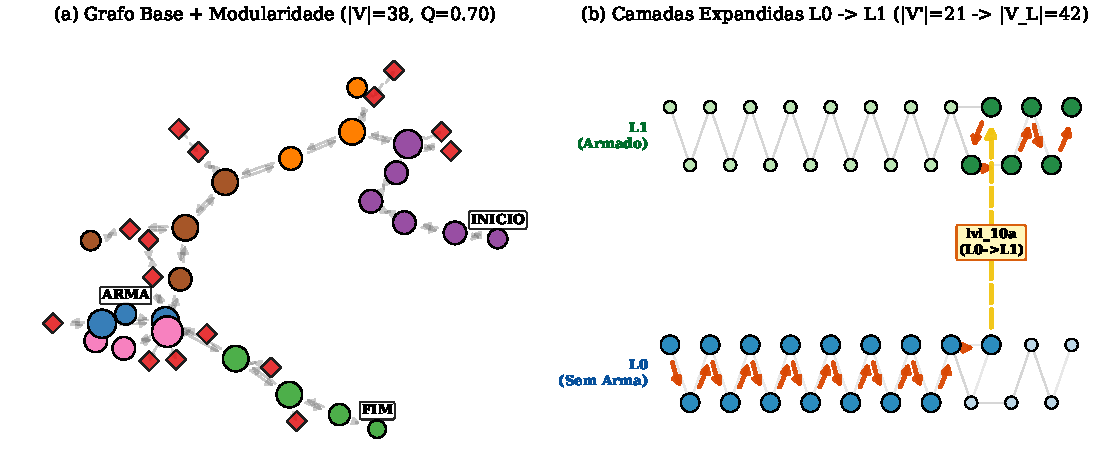
\includegraphics[width=\columnwidth]{figures/gephi_camadas_macro.pdf}
\caption{Visualiza\c{c}\~ao topol\'ogica de \textit{1-Forsaken City} no padr\~ao Gephi: (a) grafo original colorido por comunidades de modularidade (Louvain, $Q=0{,}70$) e becos contra\'iveis em vermelho; (b) grafo expandido em camadas $L_0 \to L_1$ destacando a transi\c{c}\~ao de arma em \texttt{lvl\_10a}.}
\label{fig:gephi_macro}
\end{figure}

A Tabela~\ref{tab:gephi} consolida as m\'etricas estruturais obtidas sobre os arquivos GEXF. Em todos os n\'iveis individuais, a densidade mant\'em-se reduzida ($0{,}0156$ a $0{,}0800$) com grau m\'edio pr\'oximo a $k_{\text{m\'ed}} \approx 4{,}0$, indicando topologias esparsas de corredor com ramifica\c{c}\~oes locais. Ao expandir \textit{7-The Summit} em camadas ($|V_L|=126, |E_L|=245$), a modularidade cresce para $Q = 0{,}8410$ em 13 comunidades, e nos grafos unificados por dom\'inio atinge $Q = 0{,}9288$ (\textit{Celeste}) e $Q = 0{,}8927$ (\textit{Cuphead}), refletindo forte compartimentaliza\c{c}\~ao que explica o custo combinat\'orio de buscas sem poda.

\begin{table}[htbp]
\caption{M\'etricas Topol\'ogicas Extra\'idas via Padr\~ao Gephi/Louvain}
\label{tab:gephi}
\centering
\scriptsize
\setlength{\tabcolsep}{3.5pt}
\begin{tabular}{lrrrrrr}
\toprule
\textbf{Rede GEXF} & $|V|$ & $|E|$ & $k_{\text{m\'ed}}$ & \textbf{Comun.} & \textbf{Mod. ($Q$)} & \textbf{Dens.} \\
\midrule
1-Forsaken City (Base)     &  38 &  74 & 3,89 &  6 & 0,6984 & 0,0526 \\
1-Forsaken City (Camadas)  &  42 &  81 & 3,86 &  7 & 0,7140 & 0,0470 \\
7-The Summit (Base)        &  97 & 190 & 3,92 & 10 & 0,8027 & 0,0204 \\
7-The Summit (Camadas)     & 126 & 245 & 3,89 & 13 & 0,8410 & 0,0156 \\
2-2F Funhouse (Base)       &  26 &  52 & 4,00 &  5 & 0,5889 & 0,0800 \\
2-2F Funhouse (Camadas)    &  42 &  85 & 4,05 &  5 & 0,6312 & 0,0494 \\
\textit{Celeste} Unificado & 429 & 827 & 3,86 & 25 & 0,9288 & 0,0045 \\
\textit{Cuphead} Unificado & 152 & 300 & 3,95 & 15 & 0,8927 & 0,0131 \\
\bottomrule
\end{tabular}
\end{table}

Na Figura~\ref{fig:contracao}, quantifica-se a redu\c{c}\~ao de v\'ertices pela contra\c{c}\~ao iterativa de becos nas 14 fases reais. Em mapas com densas ramifica\c{c}\~oes secund\'arias como \textit{Old Site} (C2), \textit{Mirror Temple} (C5) e \textit{Celestial Resort} (C3), a contra\c{c}\~ao eliminou 72,7\% ($33 \to 9$), 66,7\% ($45 \to 15$) e 64,6\% ($65 \to 23$) das salas antes da expans\~ao em camadas.

\begin{figure}[htbp]
\centering
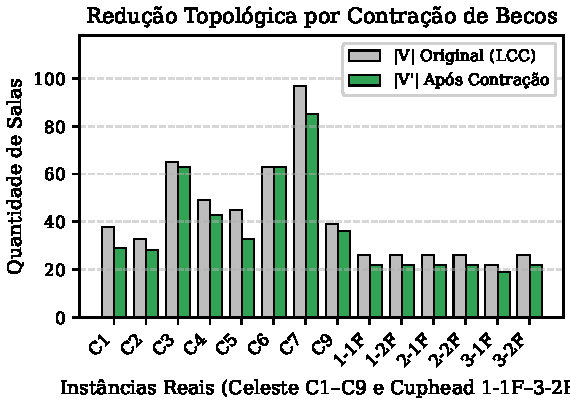
\includegraphics[width=0.95\columnwidth]{figures/contracao_becos.pdf}
\caption{Redu\c{c}\~ao do n\'umero de salas ($|V| \to |V'|$) obtida pela contra\c{c}\~ao topol\'ogica de becos sem sa\'ida nos mapas de \textit{Celeste} e \textit{Cuphead}.}
\label{fig:contracao}
\end{figure}

\subsection{Compara\c{c}\~ao de Rotas: Custo Real e Peso Efetivo}
Para responder de forma rigorosa \`a compara\c{c}\~ao com o \textit{baseline} BFS sem depender exclusivamente do peso heur\'istico (\ref{eq:peso_efetivo}), as Tabelas~\ref{tab:celeste} e~\ref{tab:cuphead} reportam conjuntamente o \textbf{Custo Real} ($\text{TempoBase} + \text{Dificuldade}$) e o \textbf{Peso Efetivo} nos 8 cap\'itulos de \textit{Celeste} e nas 6 fases de \textit{Cuphead}, complementadas visualmente pelas Figuras~\ref{fig:custos} e~\ref{fig:gephi_rota}.

Mesmo sob a m\'etrica f\'isica n\~ao descontada (\textbf{Custo Real}), o Dijkstra em Camadas supera expressivamente o BFS em todas as 14 inst\^ancias reais: reduz o custo real entre \textbf{11,1\%} (\textit{Forsaken City}) e \textbf{50,9\%} (\textit{Reflection}) em \textit{Celeste} (com queda de \textbf{48,1\%} em \textit{The Summit}), e entre \textbf{55,4\%} (\textit{Funfair Fever}) e \textbf{68,3\%} (\textit{Funhouse Frazzle}) em \textit{Cuphead}, acompanhado de redu\c{c}\~oes de peso efetivo de at\'e 52,5\% e 67,9\%, respectivamente. Como todos os itens opcionais das 14 fases reais residem em ramifica\c{c}\~oes terminais ou sobre o eixo percorrido, a contra\c{c}\~ao assegura coleta de 100\% nessas fases --- enquanto a abla\c{c}\~ao sem contra\c{c}\~ao (\texttt{--no-contract}) deixa para tr\'as mais da metade dos itens em \textit{Celeste} (ex.: 19/41 em \textit{The Summit}) e todas as 5 moedas douradas em todas as fases de \textit{Cuphead}.

\begin{table*}[htbp]
\caption{Desempenho Comparativo nos 8 Cap\'itulos Oficiais de \textit{Celeste} ($\alpha = 0{,}05$)}
\label{tab:celeste}
\centering
\scriptsize
\setlength{\tabcolsep}{4.0pt}
\begin{tabular}{lrrrrrrrrrr}
\toprule
\textbf{Cap\'itulo} & $|V|\to|V'|$ & \textbf{BFS Real} & \textbf{Dijk. Real} & \textbf{Red. Real} & \textbf{BFS Efet.} & \textbf{Dijk. Efet.} & \textbf{Red. Efet.} & \textbf{Itens (B/D/NC)} & \textbf{Dijk. (ms)} & \textbf{DFS (ms)} \\
\midrule
1-Forsaken City    & 38 $\to$ 21 &   746,7 &   664,1 & 11,1\% &   533,1 &   466,5 & 12,5\% & 21/21/9  & 0,045 & 0,097 \\
2-Old Site         & 33 $\to$ 9  & 2.440,5 & 1.385,2 & 43,2\% &   845,4 &   473,0 & 44,1\% & 18/18/1  & 0,022 & 0,042 \\
3-Celestial Resort & 65 $\to$ 23 & 2.540,4 & 1.456,2 & 42,7\% &   989,3 &   545,5 & 44,9\% & 24/24/7  & 0,056 & 0,123 \\
4-Golden Ridge     & 49 $\to$ 35 & 1.549,2 & 1.019,0 & 34,2\% &   936,9 &   557,8 & 40,5\% & 29/29/16 & 0,089 & 0,198 \\
5-Mirror Temple    & 45 $\to$ 15 & 1.981,7 & 1.234,0 & 37,7\% &   742,1 &   442,9 & 40,3\% & 22/22/1  & 0,041 & 0,095 \\
6-Reflection       & 63 $\to$ 48 &   910,5 &   447,3 & 50,9\% &   882,6 &   419,4 & 52,5\% &  2/2/0   & 0,117 & 0,310 \\
7-The Summit       & 97 $\to$ 63 & 3.308,3 & 1.715,6 & 48,1\% & 2.395,3 & 1.229,3 & 48,7\% & 41/41/19 & 0,174 & 0,461 \\
9-Core             & 39 $\to$ 30 &   835,3 &   497,4 & 40,4\% &   651,1 &   343,9 & 47,2\% &  7/7/2   & 0,081 & 0,217 \\
\bottomrule
\multicolumn{11}{l}{\tiny Itens (B/D/NC): BFS c/ contra\c{c}\~ao / Dijkstra c/ contra\c{c}\~ao / abla\c{c}\~ao Dijkstra sem contra\c{c}\~ao (\texttt{--no-contract}).}
\end{tabular}
\end{table*}

\begin{table*}[htbp]
\caption{Desempenho Comparativo nas 6 Fases \textit{Run-and-Gun} de \textit{Cuphead} ($\alpha = 0{,}05$)}
\label{tab:cuphead}
\centering
\scriptsize
\setlength{\tabcolsep}{4.0pt}
\begin{tabular}{lrrrrrrrrrr}
\toprule
\textbf{Fase (\textit{Isle})} & $|V|\to|V'|$ & \textbf{BFS Real} & \textbf{Dijk. Real} & \textbf{Red. Real} & \textbf{BFS Efet.} & \textbf{Dijk. Efet.} & \textbf{Red. Efet.} & \textbf{Itens (B/D/NC)} & \textbf{Dijk. (ms)} & \textbf{DFS (ms)} \\
\midrule
1-1F Forest Follies  & 26 $\to$ 21 &   611,5 & 267,7 & 56,2\% &   490,9 & 210,0 & 57,2\% & 5/5/0 & 0,064 & 0,356 \\
1-2F Treetop Trouble & 26 $\to$ 21 & 1.478,5 & 497,2 & 66,4\% & 1.252,6 & 402,2 & 67,9\% & 5/5/0 & 0,063 & 0,637 \\
2-1F Funfair Fever   & 26 $\to$ 21 &   577,9 & 257,8 & 55,4\% &   461,9 & 205,2 & 55,6\% & 5/5/0 & 0,073 & 0,437 \\
2-2F Funhouse Frazz. & 26 $\to$ 21 & 2.100,5 & 666,9 & 68,3\% & 1.662,2 & 532,9 & 67,9\% & 5/5/0 & 0,061 & 0,334 \\
3-1F Perilous Piers  & 22 $\to$ 17 & 1.246,4 & 411,3 & 67,0\% &   968,2 & 320,7 & 66,9\% & 5/5/0 & 0,038 & 0,084 \\
3-2F Rugged Ridge    & 26 $\to$ 21 & 1.268,1 & 540,5 & 57,4\% & 1.059,7 & 429,2 & 59,5\% & 5/5/0 & 0,060 & 0,286 \\
\bottomrule
\multicolumn{11}{l}{\tiny Itens (B/D/NC): BFS c/ contra\c{c}\~ao / Dijkstra c/ contra\c{c}\~ao / abla\c{c}\~ao Dijkstra sem contra\c{c}\~ao (\texttt{--no-contract}).}
\end{tabular}
\end{table*}

\begin{figure*}[htbp]
\centering
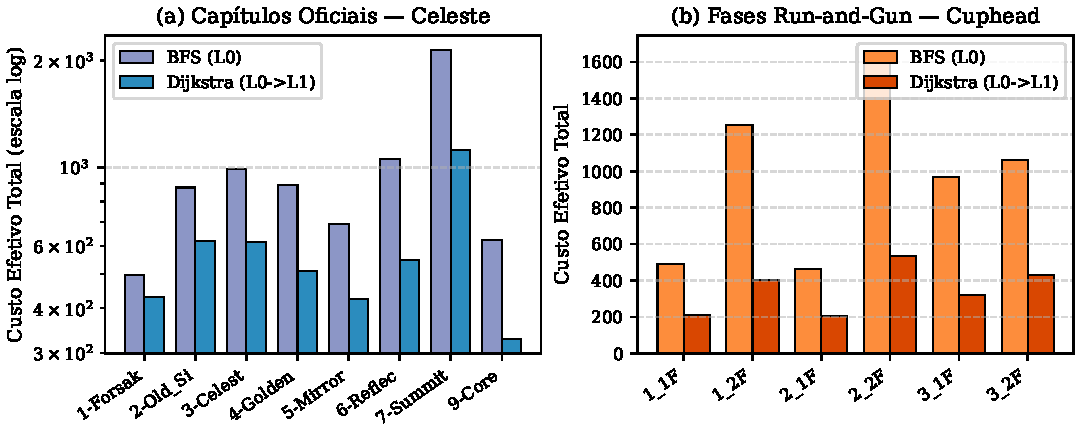
\includegraphics[width=0.92\textwidth]{figures/comparacao_custos.pdf}
\caption{Compara\c{c}\~ao do Peso Efetivo Total entre o \textit{baseline} BFS (Camada $L_0$) e o Dijkstra no Grafo Expandido em Camadas ($L_0 \to L_1$) nos 8 cap\'itulos de \textit{Celeste} e nas 6 fases de \textit{Cuphead}.}
\label{fig:custos}
\end{figure*}

A Figura~\ref{fig:gephi_rota} evidencia por filtragem visual de subgrafo em \textit{2-2F Funhouse Frazzle} a razão dessa economia real de 68,3\%: enquanto o BFS atravessa toda a espinha na camada $L_0$ sob alta dificuldade acumulada (Fig.~\ref{fig:gephi_rota}a), o Dijkstra em camadas desvia no in\'icio do mapa at\'e a sala de melhoria \textit{Parry Shrine}, salta para $L_1$, aproveita a rota elevada subsequente e reduz o custo real total de $2.100{,}5$ para $666{,}9$.

\begin{figure}[htbp]
\centering
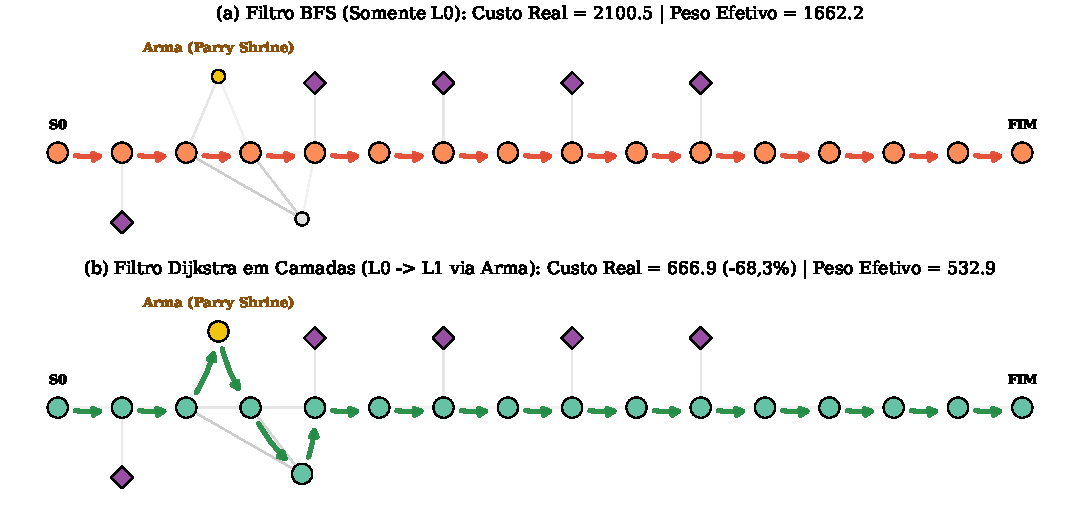
\includegraphics[width=\columnwidth]{figures/gephi_rota_comparativa.pdf}
\caption{Filtragem visual das rotas em \textit{2-2F Funhouse Frazzle}: (a) rota direta do BFS restrita \`a camada $L_0$; (b) desvio estrat\'egico do Dijkstra pela sala \textit{Parry Shrine} ($L_0 \to L_1$), capturando as 5 moedas contra\'idas com corte de 68,3\% no custo real.}
\label{fig:gephi_rota}
\end{figure}

Cumpre esclarecer que, nas 14 fases reais e nos grafos sint\'eticos com $|V| \le 30$, o Dijkstra e o DFS \textit{Branch-and-Bound} coincidiram numericamente em custo real e efetivo porque nenhuma sala portadora de colet\'avel (nem n\'o pai contra\'ido) foi cruzada simultaneamente em $L_0$ e $L_1$ na rota \'otima. Em topologias c\'iclicas arbitr\'arias nas quais uma sala colet\'avel intermedi\'aria sirva tanto na ida ($L_0$) quanto no retorno ap\'os a arma ($L_1$) --- fen\^omeno observado isoladamente na inst\^ancia sint\'etica \texttt{v\_0060} ---, a soma est\'atica sobre $G_L$ otimizada pelo Dijkstra considera o desconto da sala nas duas passagens, enquanto \texttt{evaluate\_path} e o DFS \textit{Branch-and-Bound} deduplicam o incentivo por sala. Essa diverg\^encia pontual decorre diretamente da escolha polinomial de n\~ao embutir bitmasks de itens no estado do grafo em camadas.

\subsection{Sensibilidade do Par\^ametro $\alpha$ e Escalabilidade Assint\'otica}
A Figura~\ref{fig:sensibilidade} avalia o par\^ametro heur\'istico $\alpha \in \{0{,}00, 0{,}02, 0{,}05, 0{,}10, 0{,}25, 0{,}50\}$ na inst\^ancia sint\'etica \texttt{v\_0150}, que possui ciclos paralelos e itens fora de becos terminais. Sem depender de compara\c{c}\~oes diretas entre pesos substitutos de grafos topologicamente distintos, observa-se no painel~(a) que o aumento de $\alpha$ eleva monotonicamente os itens capturados com contra\c{c}\~ao de $30$ ($\alpha=0{,}00$, valor acumulado $274{,}4$) para $43$ ($\alpha=0{,}50$, valor $402{,}6$), ao passo que a vers\~ao \texttt{--no-contract} estagna em apenas $17$ itens ($132{,}7$). No painel~(b), o custo real com contra\c{c}\~ao cresce apenas $5{,}9\%$ (de $1.288{,}6$ para $1.364{,}3$) para entregar $+43{,}3\%$ mais itens, enquanto o peso efetivo decai conforme o denominador heur\'istico $(1 + \alpha \cdot \text{ValorColetavel})$, demonstrando que $\alpha$ atua como controlador est\'avel de desvios por recompensas sem violar a estabilidade do caminho m\'inimo.

\begin{figure}[htbp]
\centering
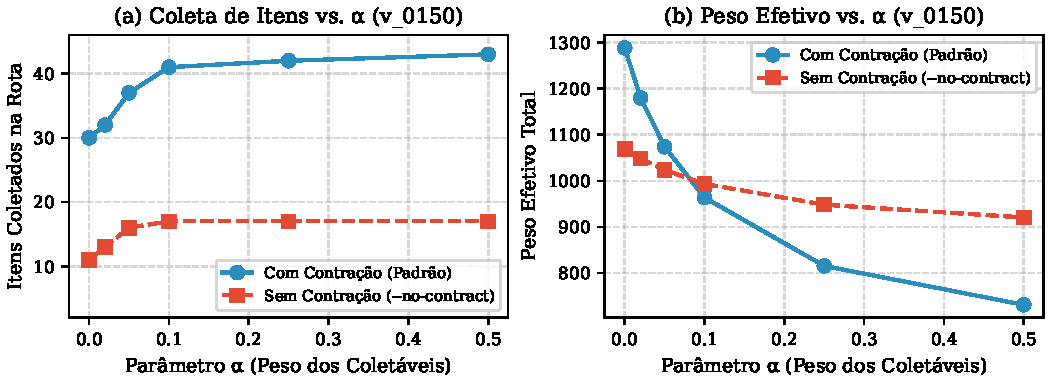
\includegraphics[width=0.98\columnwidth]{figures/sensibilidade_alpha.pdf}
\caption{An\'alise de sensibilidade de $\alpha$ em \texttt{v\_0150}: (a) itens coletados vs. $\alpha$; (b) comportamento do custo real e do peso efetivo frente \`a abla\c{c}\~ao \texttt{--no-contract}.}
\label{fig:sensibilidade}
\end{figure}

Para avaliar o comportamento assint\'otico sob crescimento da entrada, a Tabela~\ref{tab:sinteticos} e a Figura~\ref{fig:escalabilidade} re\'unem os resultados de $|V|=15$ a $|V|=5.000$. Observa-se o gargalo combinado do \textit{Branch-and-Bound}: embora iguale o resultado de $L_0 \to L_1$ at\'e $|V|=30$ (expandindo 943 estados em 2,30~ms), a ramifica\c{c}\~ao exponencial por ciclos paralelos faz o algoritmo atingir o limite de 150~ms j\'a em $|V|=60$ ap\'os mais de 65.000 visitas. Em contraste, o Dijkstra em camadas respeita a cota $O((V+E)\log V)$, solucionando o grafo de 5.000 salas (8.000 estados em $G_L$ ap\'os contra\c{c}\~ao de 1.000 becos) em 14,49~ms e 5.238 estados. Nota-se ainda que nos benchmarks sint\'eticos, como h\'a itens dispostos em rotas paralelas disjuntas do eixo principal, nem o Dijkstra nem o DFS atingem 100\% dos colet\'aveis do grafo inteiro --- confirmando que a garantia de 100\% de cobertura da contra\c{c}\~ao restringe-se exclusivamente aos itens situados em becos terminais ligados aos v\'ertices visitados.

\begin{table}[htbp]
\caption{Escalabilidade Assint\'otica nos Grafos Sint\'eticos ($\alpha = 0{,}05$)}
\label{tab:sinteticos}
\centering
\scriptsize
\setlength{\tabcolsep}{2.8pt}
\begin{tabular}{rrrrrrr}
\toprule
$|V|$ \textbf{Orig.} & $|V'|$ \textbf{Contr.} & \textbf{BFS (ms)} & \textbf{Dijk. (ms)} & \textbf{DFS B\&B (ms)} & \textbf{Est. Dijk.} & \textbf{Est. DFS} \\
\midrule
  15 &   12 &  0,02 &  0,04 &   0,21 &    19 &     84 \\
  30 &   24 &  0,05 &  0,08 &   2,30 &    32 &    943 \\
  60 &   48 &  0,09 &  0,15 & 150,08* &    68 & 71.104 \\
 150 &  120 &  0,22 &  0,34 & 150,13* &   163 & 68.544 \\
 500 &  400 &  0,69 &  1,07 & 150,35* &   527 & 71.040 \\
1500 & 1200 &  2,98 &  4,66 & 150,91* & 1.578 & 66.560 \\
5000 & 4000 & 11,32 & 14,49 & 153,07* & 5.238 & 65.792 \\
\bottomrule
\multicolumn{7}{l}{\tiny *Execu\c{c}\~ao interrompida pelo limite de seguran\c{c}a (\textit{timeout} de 150~ms).}
\end{tabular}
\end{table}

\begin{figure}[htbp]
\centering
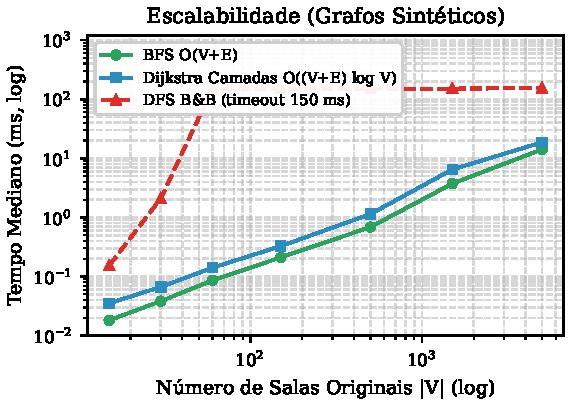
\includegraphics[width=0.95\columnwidth]{figures/escalabilidade_tempo.pdf}
\caption{Curva de escalabilidade em escala log-log comparando o tempo mediano de execu\c{c}\~ao (ms) de BFS, Dijkstra em Camadas e DFS \textit{Branch-and-Bound} para $|V| \in [15, 5000]$.}
\label{fig:escalabilidade}
\end{figure}

% ============================================================================
\section{Conclus\~ao e Pr\'oximas Etapas}
\label{sec:conclusao}
% ============================================================================

Este trabalho apresentou o \textit{StratGraph}, demonstrando que a combina\c{c}\~ao entre contra\c{c}\~ao topol\'ogica de becos sem sa\'ida e expans\~ao markoviana em duas camadas ($L_0 \to L_1$) soluciona em tempo polinomial $O((V+E)\log V)$ o objetivo substitutivo estrat\'egico de desvio por equipamento e captura de alcovas colet\'aveis. Validado em 14 mapas reais e 7 redes sint\'eticas --- al\'em de an\'alise modular no Gephi ($Q$ entre $0{,}59$ e $0{,}93$) ---, o m\'etodo reduziu em at\'e 50,9\% o custo real em \textit{Celeste} e at\'e 68,3\% em \textit{Cuphead} frente ao BFS com id\^entica cobertura de 100\% dos itens, superando de forma decisiva o gargalo exponencial do \textit{Branch-and-Bound} a partir de $|V|=60$.

Como limita\c{c}\~oes claras da arquitetura atual e dire\c{c}\~oes para trabalhos futuros, destacam-se quatro frentes:
\begin{enumerate}
    \item \textbf{Relaxa\c{c}\~ao sem bitmask de colet\'aveis:} Embora mantenha a complexidade polinomial $O(2|V|)$, o grafo em camadas est\'atico permite desconto duplo caso uma sala colet\'avel intermedi\'aria ou n\'o contra\'ido seja cruzado em $L_0$ e depois em $L_1$, justificando investigar algoritmos rotulados (\textit{label-setting}) restritos apenas aos n\'os articuladores de passagem dupla.
    \item \textbf{Extens\~ao para m\'ultiplas ferramentas ($k$ camadas):} Jogos ou redes log\'isticas com $k$ equipamentos independentes exigem $2^k|V|$ estados, motivando o uso de heur\'isticas admiss\'iveis com busca $A^*$ informada.
    \item \textbf{Abstra\c{c}\~ao topol\'ogica discreta por sala:} Os pesos sintetizam o custo de travessia em escalares por sala/plataforma; integrar modelos din\^amicos de cinem\'atica cont\'inua refinaria as estimativas de tempo.
    \item \textbf{S\'intese procedural balanceada:} Aplicar as m\'etricas de modularidade do Gephi e a raz\~ao entre rotas $L_0$ e $L_1$ como fun\c{c}\~ao objetivo na gera\c{c}\~ao procedural de fases com desvios t\'aticos bem calibrados.
\end{enumerate}

% ============================================================================
\section{Algoritmo e Base de Dados}
\label{sec:disponibilidade}
% ============================================================================

Em conformidade com os crit\'erios de reprodutibilidade aberta e execu\c{c}\~ao nativa via terminal em ambiente Linux (Ubuntu~24.04), o c\'odigo-fonte modular em Python~3.12 (biblioteca padr\~ao em \texttt{src/}), os scripts de experimentos e exporta\c{c}\~ao GEXF e a su\'ite de testes automatizados encontram-se publicamente dispon\'iveis no reposit\'orio GitHub em~\cite{repo_codigo}. Todos os 22 grafos estruturados em CSV (\textit{Celeste}, \textit{Cuphead}, \textit{benchmarks} sint\'eticos e \textit{sample\_toy}), acompanhados dos resumos experimentais e documenta\c{c}\~ao do esquema, est\~ao preservados com identificador persistente DOI no reposit\'orio Zenodo em~\cite{dataset_zenodo}.

\bibliographystyle{IEEEtran}
\bibliography{references}

\end{document}
